\section{Funktionsweise von Vektoruhren}
\subsection{Prinzipielle Funktionsweise}

Wie bereits beschrieben wurde, bilden Vektoruhren eine Erweiterung der Lamportuhr. Dabei wird in jedem Prozess im System ein Integer als Zähler in der Vektoruhr gespeichert. Im Allgemeinen werden durch eine Vektoruhr Zeitstempel mit Events im System assoziiert \cite{Baldoni:2002:FDC:1435723.1437765}[S. 3].

Jeder Prozess im System besitzt seine eigene Vektoruhr in der Form eines Vektors $VC_i[1...n]$, wobei alle Elemente der Uhr mit $0$ initialisiert werden. Die Uhr eines Prozesses wird wie folgt verwaltet und aktualisiert:

\begin{itemize}
	\item[R1]Jedes mal, wenn ein Prozess $P_i$ ein Event auslöst, muss dieser seine Vektoruhr für den Eintrag $VC_i$ um Eins hochzählen, es gilt  $VC_i[i] := VC_i[i] + 1$. Dadurch verdeutlicht der Prozess, dass er etwas getan hat und signalisiert dies den anderen Prozessen durch aktualisieren seiner Vektoruhr 
	\item[R2]Sendet ein Prozess $P_i$ eine Nachricht $m$, so hängt er seine aktuelle Vektoruhr $VC_i$ an die zu sendende Nachricht an. Auf diese Weise gelangt die Uhr zu dem Empfänger der Nachricht.
	\item[R3]Empfängt ein Prozess $P_i$ eine Nachricht, so muss er seine Vektoruhr aktualisieren. Dabei geht er wie folgt vor: $VC_i = \max(VC_i, m.VC)$. Dies bedeutet, dass der Prozess für jedes Element seiner Vektoruhr überprüft ob der Wert in der Uhr der Nachricht größer als der eigene ist. Sollte dies der Fall sein, wird der eigene Wert an dieser Stelle mit dem Wert aus der anderen Uhr überschrieben.\label{R3}
\end{itemize} \cite{Baldoni:2002:FDC:1435723.1437765}[S. 4]

Die Werte innerhalb einer Vektoruhr $VC_i$ haben eine besondere Bedeutung für den Prozess $P_i$. $VC_i[i]$ gibt die Anzahl an Events an, welche $P_i$ zu dem Zeitpunkt des Betrachtens verarbeitet hat. Die anderen Werte der Uhr ($VC_i[j]$ mit $j \neq i$) zeigen an, dass alle Events welche durch den Prozess $P_j$ verarbeitet wurden, sich kausal betrachtet in der Vergangenheit von $P_i$ befinden. Sie geben sozusagen an, was der Prozess $P_i$ über die Zeiten der anderen Prozesse weiß, diese Information kann sich zu dem Zeitpunkt jedoch bereits von den tatsächlichen Zeiten unterscheiden. Da jeder Prozess lediglich seinen Zähler in der Vektoruhr erhöhen darf, hat dieser Prozess zu jedem Zeitpunkt den aktuellsten Stand seiner lokalen Zeit. \cite{SINGHAL199247}[S. 48]

\subsubsection{Vergleich von Vektoruhren untereinander}
Eine Besonderheit der Vektoruhren besteht im Vergleich von Uhren untereinander. Dies wird notwendig, sobald ein Prozess eine Nachricht erhält und diese verarbeiten muss. Wie in Bedingung R3 unter \ref{R3} - \nameref{R3} zu sehen, muss der Prozess seine Uhr entsprechen der mitgeschickten Vektoruhr der Nachricht aktualisieren. Der Vergleich zwischen der eigenen und der empfangenen Uhr muss dann auf Anwendungsebene geschehen, denn dort wird entschieden was mit der angekommenen Nachricht geschieht.

Für zwei zu vergleichende Uhren $VC_1$ und $VC_2$ gibt es folgenden Beziehungen:

\begin{eqnarray}
&VC_1 \leq VC_2& \text{ wenn } \forall i : VC_1[i] \leq VC_2[i] \\
	&VC_1 < VC_2& \text{ wenn } VC_1 \leq VC_2 \text{ \& } VC_1 \neq VC_2 \\
	&VC_1 \mid \mid VC_2& \text{ wenn } !(VC_1 < VC_2) \text{ \& } !(VC_2 < VC_1)
\end{eqnarray}
\cite{Mattern88virtualtime}[S. 127, Definition 4]

Fall (1) bedeutet, dass eine Uhr $VC_1$ kleiner oder gleich $VC_2$ ist, wenn jedes Element von $VC_1$ kleiner oder gleich dem entsprechenden Element in $VC_2$ ist. Der zweite Fall (2) liegt vor, wenn Fall (1) zutrifft und zusätzlich kein Element in $VC_1$ gleich dem entsprechenden Element in $VC_2$ ist. 
Der letzte Fall (3) ist ein Besonderer Fall. Dieser trifft ein wenn nicht entschieden werden kann, welche Uhr neuer oder älter beziehungsweise nach der obigen Definition größer oder kleiner ist als die andere. Die entsprechenden Nachrichten wurden sozusagen gleichzeitig abgeschickt. Dieser im Englischen als \glqq Concurrent\glqq{} bezeichnete Fall stellt ein großes Problem für Systeme dar, die Vektoruhren für die zeitliche Synchronisation der Kommunikation nutzen. Auf diesen Sonderfall wird im nächsten Kapitel genauer eingegangen.
\subsubsection{Beispiel einer Kommunikation}
Um die Funktionsweise von Vektoruhren genauer zu beschreiben, wird nun anhand eines einfachen Beispieles die Kommunikation in einem System mit drei Prozessen sowie die Verarbeitung der Vektoruhren eines jeden Prozesses gezeigt.

\begin{figure}[ht]
	\centering
	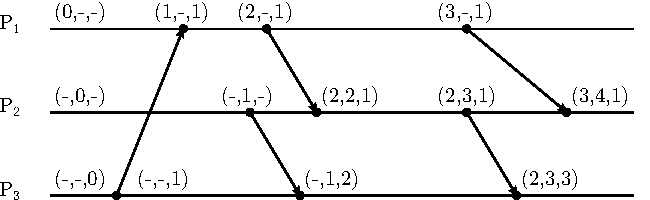
\includegraphics[width=12cm]{KommBeispiel1.pdf}
	\caption[Beispiel einer Kommunikation]{Ablauf der Kommunikation dreier Prozesse mit Veranschaulichung der dabei auftretenden Vektoruhren}
	Quelle: Nachgezeichnet aus \cite{Baldoni:2002:FDC:1435723.1437765}
\label{figure:kommBeispiel1}
\end{figure}
\FloatBarrier

Zu Beginn weiß jeder Prozess nur seine lokale Zeit, der Wert $VC_i$ für Prozess $P_i$ wird deshalb auf $0$ gesetzt. Da der Prozess noch keine Kenntnis über die anderen Teilnehmer im System hat, werden die anderen Einträge mit \glqq$-$\glqq{} initialisiert.

Zu Beginn sendet in dem in Abbildung \ref{figure:kommBeispiel1} abgebildeten Beispiel Prozess $P_3$ eine Nachricht an $P_1$. Er erzeugt dabei ein Event und muss deshalb zunächst seine lokale Vektoruhr inkrementieren, der Wert $VC_3[3]$ wird also um $1$ erhöht. Die Uhr hat nun den Wert \vc{-}{-}{1}. Anschließend wird die lokale Uhr an die zu sendende Nachricht angehängt und diese verschickt.
Nun empfängt Prozess $P_1$ diese Nachricht. Gemäß Regel R1 muss zunächst die lokale Uhr entsprechend der mitgeschickten Uhr aktualisiert werden. Da in jedem Feld der Uhr das Maximum genommen wird, wird die lokale Uhr von $P_1$ nach der Aktualisierung von \vc{0}{-}{-} auf \vc{1}{-}{1} geändert. Da das Empfangen einer Nachricht auch als Event angesehen wird, erhöht sich auch der Wert für den lokalen Zähler von $P_1$ innerhalb der Uhr um $1$.

In diesem Beispiel kommen alle Nachrichten passend nacheinander an und es kann zu keinen Konflikten in der Ausführungsreihenfolge kommen. Das Nachfolgende Beispiel verdeutlicht den Fall, dass Gesendete Nachrichten auch von anderen Nachrichten abhängig und während der Übertragung verzögert ankommen können, was ein Problem eines einfachen Systems mit Vektoruhren darstellt.




\subsection{Umsetzung in C\#}
Für die Umsetzung dieses Themas wurde C\# als Programmiersprache ausgewählt. Damit die zeitliche Synchronisation mittels Vektoruhren möglichst realitätsnah simuliert werden kann, wurden drei virtuelle Maschinen mit dem Betriebssystem Windows 8.1 aufgesetzt. Diese befinden sich im Hochschulnetzwerk und können per Remote Desktop bedient werden.

Die Implementierung wurde in zwei unabhängige Programmteile aufgeteilt. Diese sind ein Commander sowie Nodes. 

TODO: Abbildung des Gesamtsystemes (Commander + 3 Nodes)

Der Commander stellt sozusagen eine übergeordnete Kommandozentrale dar, welche die Kommunikation der Nodes untereinander durch gewisse Steuerbefehle koordiniert. Er besitzt eine grafische Oberfläche, welche mittels WPF erstellt wurde.

\begin{figure}[ht]
	\centering
	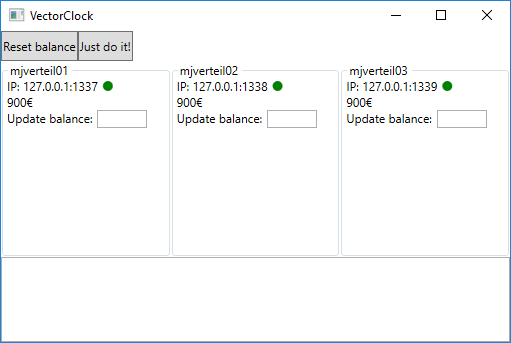
\includegraphics[width=10cm]{commanderWindow.png}
	\caption[Commander Window]{Abbildung des Commanderfensters, welcher dazu dient, die Kommunikation zwischen den Nodes durch Steuerbefehle zu koordinieren}
	\label{figure:commanderWindow}
\end{figure}
\FloatBarrier

Ein Node stellt einen Knoten in dem simulierten System dar. In diesem werden Events ausgeführt und Vektoruhren verarbeitet. Jeder Node besitzt seine eigene, lokale Vektoruhr. Bei einem Node handelt es sich um ein Kommandozeilenprogramm, welches auf einer VM läuft und ständig auf Nachrichten wartet. Damit der Ablauf der Kommunikation besser nachvollzogen werden kann, gibt ein Node bei jedem Event die Details der Nachricht sowie seiner Vektoruhr aus. Zusätzlich sendet er dabei eine Antwort an den Commander mit der Nachricht, welche er erhalten hat und seiner aktuellen lokalen Uhr. Der Commander gibt diese empfangene Antwort in einem Textfenster aus.

\begin{figure}[ht]
	\centering
	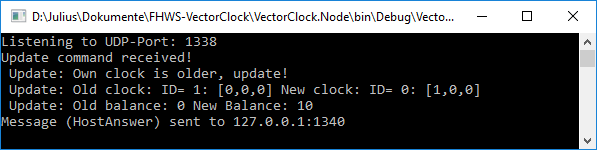
\includegraphics[width=10cm]{nodeWindow.png}
	\caption[Node Window]{Abbildung des Nodefensters. Zwischen den Nodes findet die eigentlichen Kommunikation statt.}
\label{figure:nodeWindow}
\end{figure}
\FloatBarrier

Die Kommunikation zwischen dem Commander und den Nodes wurde mittels UDP realisiert. Die Entscheidung viel auf UDP, da sich dadurch unnötiger Overhead und Programmieraufwand vermeiden lässt, welcher beispielsweise bei TCP angefallen wäre. Der Aufbau einer Nachricht ist in Abbildung \ref{Nachricht} dargestellt. Beim Absenden der Nachricht, egal ob im Commander oder in den Nodes, wird diese serialisiert und per UPD versendet. Im Empfangsfall muss der empfangene Datenstrom wieder deserialisiert und in eine Nachricht umgewandelt werden. 
